% $Header: /cvsroot/latex-beamer/latex-beamer/solutions/conference-talks/conference-ornate-20min.en.tex,v 1.6 2004/10/07 20:53:08 tantau Exp $

\documentclass{beamer}

\setbeamerfont{subsection title}{size=\LARGE}
\setbeamertemplate{subsection page}
{
  \begin{centering}
    \begin{beamercolorbox}[center]{part title}
      \usebeamerfont{subsection title}\insertsubsection\par
    \end{beamercolorbox}
  \end{centering}
}
\def\subsectionpage{\usebeamertemplate*{subsection page}}

\AtBeginSubsection{\frame{\subsectionpage}}
\mode<presentation>
{
%  \usetheme{Hannover}
\usetheme[width=0.7in]{Hannover}
% or ...

  \setbeamercovered{transparent}
  % or whatever (possibly just delete it)
}
\usepackage{longtable}
\usepackage{booktabs}
\usepackage{qtree}
\usepackage{natbib}
\usepackage[english]{babel}
% or whatever

\usepackage[latin1]{inputenc}
% or whatever

\usepackage{times}
%\usepackage[T1]{fontenc}
% Or whatever. Note that the encoding and the font should match. If T1
% does not look nice, try deleting the line with the fontenc.
%\usepackage{logictheme}

\usepackage{multirow}
\usepackage{totpages}
\usepackage{hyperref}
\usepackage{booktabs}

\usepackage{listings}
\usepackage{tikz}
\usetikzlibrary{positioning}

\newcommand{\blt}{- } %used for bullets in a list

\newcounter{datadefnum} %Datadefinition Number
\newcommand{\ddthedatadefnum}{DD\thedatadefnum}
\newcommand{\ddref}[1]{DD\ref{#1}}

\newcommand{\colAwidth}{0.1\textwidth}
\newcommand{\colBwidth}{0.8\textwidth}

\renewcommand{\arraystretch}{1.1} %so that tables with equations do not look crowded

\pgfdeclareimage[height=0.7cm]{logo}{McMasterLogo}
\title[\pgfuseimage{logo}] % (optional, use only with long paper titles)
{Literate Software and the \\ Drasil Framework}

%\subtitle
%{Include Only If Paper Has a Subtitle}

\author[Slide \thepage~of \pageref{TotPages}] % (optional, use only with lots of
                                              % authors)
{Dan Szymczak}
% - Give the names in the same order as the appear in the paper.
% - Use the \inst{?} command only if the authors have different
%   affiliation.

\institute[McMaster University] % (optional, but mostly needed)
{
  Computing and Software Department\\
  Faculty of Engineering\\
  McMaster University
}
% - Use the \inst command only if there are several affiliations.
% - Keep it simple, no one is interested in your street address.

\date[June 23, 2016] % (optional, should be abbreviation of conference name)
{Thesis Proposal Defense -- June 23, 2016}
% - Either use conference name or its abbreviation.
% - Not really informative to the audience, more for people (including
%   yourself) who are reading the slides online

\subject{computational science and engineering, software engineering, software
  quality, literate programming, software requirements specification, document
  driven design}
% This is only inserted into the PDF information catalog. Can be left
% out. 

% If you have a file called "university-logo-filename.xxx", where xxx
% is a graphic format that can be processed by latex or pdflatex,
% resp., then you can add a logo as follows:

%\pgfdeclareimage[height=0.5cm]{Mac-logo}{McMasterLogo}
%\logo{\pgfuseimage{Mac-logo}}

% Delete this, if you do not want the table of contents to pop up at
% the beginning of each subsection:
% \AtBeginSubsection[]
% {
%   \begin{frame}<beamer>
%     \frametitle{Outline}
%     \tableofcontents[currentsection,currentsubsection]
%   \end{frame}
% }

% If you wish to uncover everything in a step-wise fashion, uncomment
% the following command: 

%\beamerdefaultoverlayspecification{<+->}

\beamertemplatenavigationsymbolsempty 

% have SRS and LP open during the presentation

\begin{document}
\bibliographystyle{plain}
%%%%%%%%%%%%%%%%%%%%%%%%%%%%%%%%%%%%%%
\hoffset=-.4in %removing side bar for these frames
\begin{frame}[plain]

\titlepage

\end{frame}
\hoffset=0in %restore
%%%%%%%%%%%%%%%%%%%%%%%%%%%%%%%%%%%%%%

 \begin{frame}

 \frametitle{Literate Software and Drasil}
 \tableofcontents
 % You might wish to add the option [pausesections]

 % make like a story - the phases - reason for, why works, advantages
 % changing the history a bit to make a more rational narrative

 \end{frame}

%%%%%%%%%%%%%%%%%%%%%%%%%%%%%%%%%%%%%%

\section[Introduction]{Introduction}

%%%%%%%%%%%%%%%%%%%%%%%%%%%%%%%%%%%%%%

\subsection[Problem]{Problem}

%%%%%%%%%%%%%%%%%%%%%%%%%%%%%%%%%%%%%%

\begin{frame}

\frametitle{Information Duplication}
\begin{center}
\includegraphics[width=.6\textwidth]{Copies.jpg}
\end{center}
\begin{itemize}
\item Wastes resources
\item Reduces software quality
\end{itemize}

\end{frame}

%%%%%%%%%%%%%%%%%%%%%%%%%%%%%%%%%%%%%%

\begin{frame}[label=example]

\frametitle{Example}
\begin{center}
\begin{tikzpicture}[node distance=5mm]
  \tikzstyle{every node}=[draw,shape=rectangle, rounded corners,
    text width=7em, text centered];
  \node (srs) at (-4,0)         	{Requirements};
  \node (dd) at (-3.5,-1.2)  {\alert<3>{Design}};
  \node (src) at (-3,-2.4) 	{\alert<3>{Code}};
  \node (test) at (-2.5, -3.6)       {\alert<3>{Testing}};
\only<2-3>{\node(change) at (0,0) {Change R1};};
	\alt<2-3>{\draw [gray, ->, line width=2pt] (srs) -- (dd);}
  		{\draw [->, line width=2pt] (srs) -- (dd);}
  	\alt<2-3>{\draw [gray, ->, line width=2pt] (dd) -- (src);}
		{\draw [->, line width=2pt] (dd) -- (src);}
  	\alt<2-3>{\draw [gray, ->, line width=2pt] (src) -- (test);}
  		{\draw [->, line width=2pt] (src) -- (test);}
  \only<2-3>{
	\alt<3>{\draw [gray, ->, line width = 3pt] (srs) -- (change);}
		{\draw [->, line width = 3pt] (srs) -- (change);}
	}
  \only<3>{
	\draw [red, ->, line width = 3pt] (change) -- (dd);
	\draw [red, ->, line width = 3pt] (change) -- (src);
	\draw [red, ->, line width = 3pt] (change) -- (test);
	};
\end{tikzpicture}
\end{center}

\end{frame}

%%%%%%%%%%%%%%%%%%%%%%%%%%%%%%%%%%%%%%

\begin{frame}

\frametitle{Rational Design Process}
\begin{center}
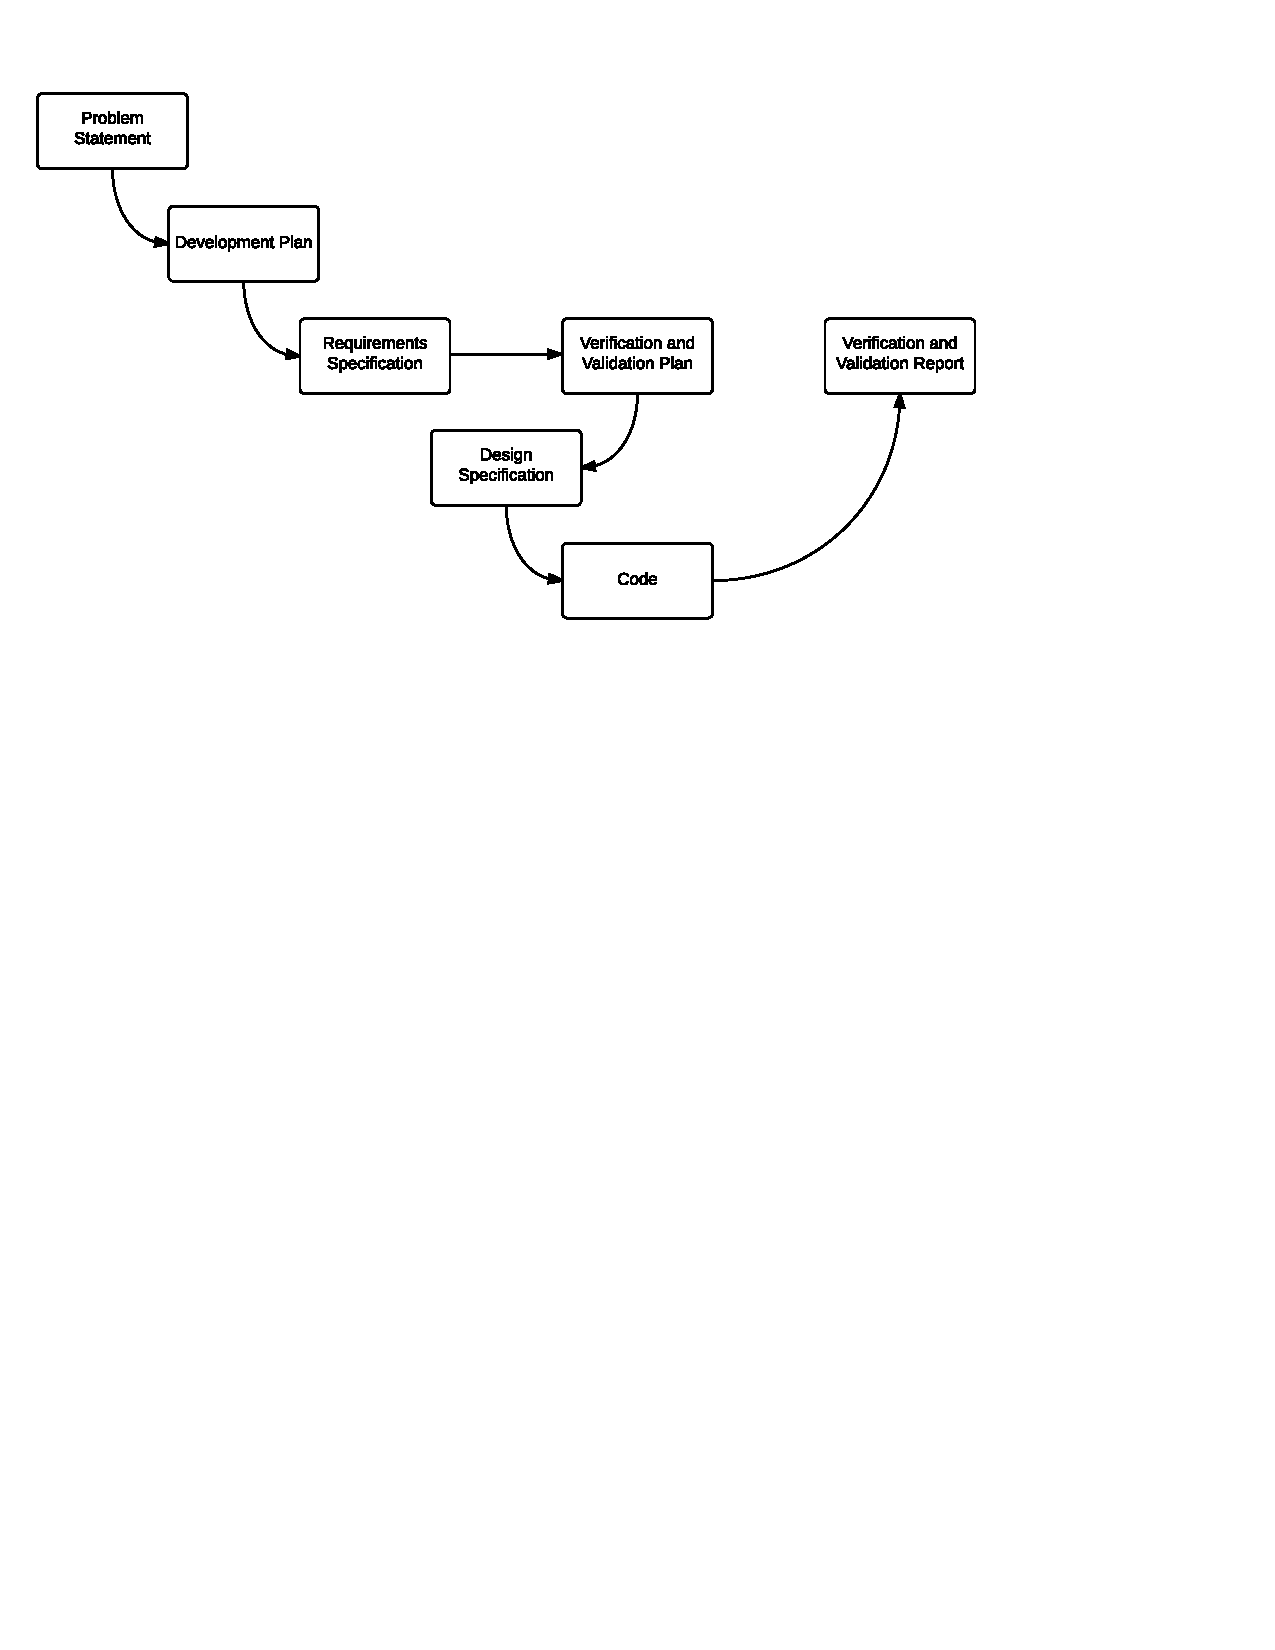
\includegraphics[width=1.02\textwidth]{OverviewOfProcess.pdf}
\end{center}

\end{frame}
%%%%%%%%%%%%%%%%%%%%%%%%%%%%%%%%%%%%%%

\begin{frame}

\frametitle{Reduced Software Qualities}

\begin{itemize}
\item{Maintainability}
\item{Traceability}
\item{Verifiability}
\item{Reproducibility}
\end{itemize}

\end{frame}

%%%%%%%%%%%%%%%%%%%%%%%%%%%%%%%%%%%%%%

\begin{frame}

\frametitle{Reproducibility}
	
\includegraphics[width=.8\textwidth]{Reproducibility.jpg}
\end{frame}

%%%%%%%%%%%%%%%%%%%%%%%%%%%%%%%%%%%%%%

\subsection[Scope]{Scope}

%%%%%%%%%%%%%%%%%%%%%%%%%%%%%%%%%%%%%%

\begin{frame}

\frametitle{Scope}

Limited to well-understood domains.
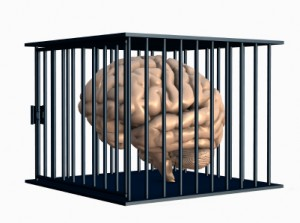
\includegraphics[width=.4\textwidth]{KC.jpg}

\only<2>{Specifically targeting Scientific Computing (SC)}
\visible<3>{Why SC?
\begin{itemize}
\item Rich, well-understood background
\item SC Developers lack software engineering background
\end{itemize}
}

\end{frame}

%%%%%%%%%%%%%%%%%%%%%%%%%%%%%%%%%%%%%%

\subsection[Goals]{Goals and Objectives}

%%%%%%%%%%%%%%%%%%%%%%%%%%%%%%%%%%%%%%

\begin{frame}

\frametitle{Goals and Objectives}

\alt<2->{Create a tool to facilitate a knowledge-based approach}
	{Simplify the development process for SC developers}
\begin{itemize}
\item Create better software artifacts
	\only<2->{\begin{itemize}\item{Ensure consistency}\end{itemize}}
\item Lower the long term cost of updating/maintaining software
	\only<2->{\begin{itemize}\item{Automate creation of software artifacts}\end{itemize}}
\item Improve reproducibility
\end{itemize}

\end{frame}

%%%%%%%%%%%%%%%%%%%%%%%%%%%%%%%%%%%%%%

\section[State of the Art]{State of The Art}

%%%%%%%%%%%%%%%%%%%%%%%%%%%%%%%%%%%%%%

\begin{frame}
\frametitle{Current Problems in SC Software Development}

\begin{itemize}
\item Emphasis on science~\cite{Kelly2007}
\item Process-heavy approaches are unfavourable~\cite{CarverEtAl2007}
\item Not enough knowledge reuse
\begin{itemize}
\item Ex. 37 of 52 triangular mesh generators implemented the same triangulation
algorithm~\cite{Owen1998}
\end{itemize}
\item Lack of understanding of software testing~\cite{Merali2010}
\item Limited tool use (especially version control~\cite{Wilson2006})
\end{itemize}

\end{frame}

%%%%%%%%%%%%%%%%%%%%%%%%%%%%%%%%%%%%%%

%\begin{frame}
%\frametitle{Generation Techniques Used in SC Software Development}
%
%Code generation has been successful in SC.
%
%\end{frame}

%%%%%%%%%%%%%%%%%%%%%%%%%%%%%%%%%%%%%

\begin{frame}
\frametitle{Literate Programming (LP)}

\begin{itemize}
\item Shifts focus to explain (to humans) what the computer should do~\cite{Knuth1984}
\item Algorithms are broken down into \emph{chunks}~\cite{JohnsonAndJohnson1997}
\item Chunks are ordered to promote understanding
\item Many tools for (or inspired by) LP
\end{itemize}

\end{frame}

%%%%%%%%%%%%%%%%%%%%%%%%%%%%%%%%%%%%%

\begin{frame}
\frametitle{Advantages of LP}

\begin{itemize}
\item Increases understandability
\item More consistent documentation and code~\cite{ShumAndCook1993}
\item Code is more maintainable~\cite{PieterseKourieAndBoake2004}
\item Code can be automatically incorporated into documentation
\item Documentation and code are updated simultaneously
\end{itemize}

\end{frame}

%%%%%%%%%%%%%%%%%%%%%%%%%%%%%%%%%%%%%

\begin{frame}
\frametitle{Drawbacks of LP}

\begin{itemize}
\item Not yet mainstream %D Mention Haskell, Agda, R, etc.
\item One-source, one document
\item Code-centric
\end{itemize}

\end{frame}

%%%%%%%%%%%%%%%%%%%%%%%%%%%%%%%%%%%%%

\begin{frame}
\frametitle{Literate Software Development (LSD)}

Combination of LP and Box Structures designed to address:

\begin{itemize}
\item Specifying interfaces between modules
\item Decomposing boxes
\item Implementing designs
\item Lack of tool support
\end{itemize}

\visible<2>{LSD's framework \emph{WebBox} addressed the above, but remains primarily \alert{code-focused}.}

\end{frame}

%%%%%%%%%%%%%%%%%%%%%%%%%%%%%%%%%%%%%

\begin{frame}
\frametitle{Reproducible Research (RR)}
\only<1>{
Reproduction can be nearly impossible without the original author's help~\cite{IonescuAndJansson2013} due to undocumented :
\begin{itemize}
\item Assumptions
\item Modifications
\item Hacks
\end{itemize}
}

\only<2>{
Compendia~\cite{GentlemanAndLang2012} provide a means of encapsulating:
\begin{itemize}
\item Research reports
\item Data
\item Code
\item ...
\end{itemize}

Compendia are intended for use in peer review.
}

\end{frame}

%D Mention: TOOL SUPPORT for RR, not compendia.

%%%%%%%%%%%%%%%%%%%%%%%%%%%%%%%%%%%%%

\section[Current Work]{Current Work}

%%%%%%%%%%%%%%%%%%%%%%%%%%%%%%%%%%%%%

\subsection[Approach]{Approach}

%%%%%%%%%%%%%%%%%%%%%%%%%%%%%%%%%%%%%

\begin{frame}

\frametitle{Knowledge Based Approach}

\only<1>{
Knowledge Capture
\begin{itemize}
\item Expand chunks
\item Specification level encapsulation
\item Easy to transform
\end{itemize}
}

\only<2,4>{
Artifact Generation
\begin{itemize}
\item Automatically update % Go beyond LP
\uncover<4>{\item Traceability \& maintainability
\item Reproducibility}
\end{itemize}
}

\only<3>{
\begin{center}
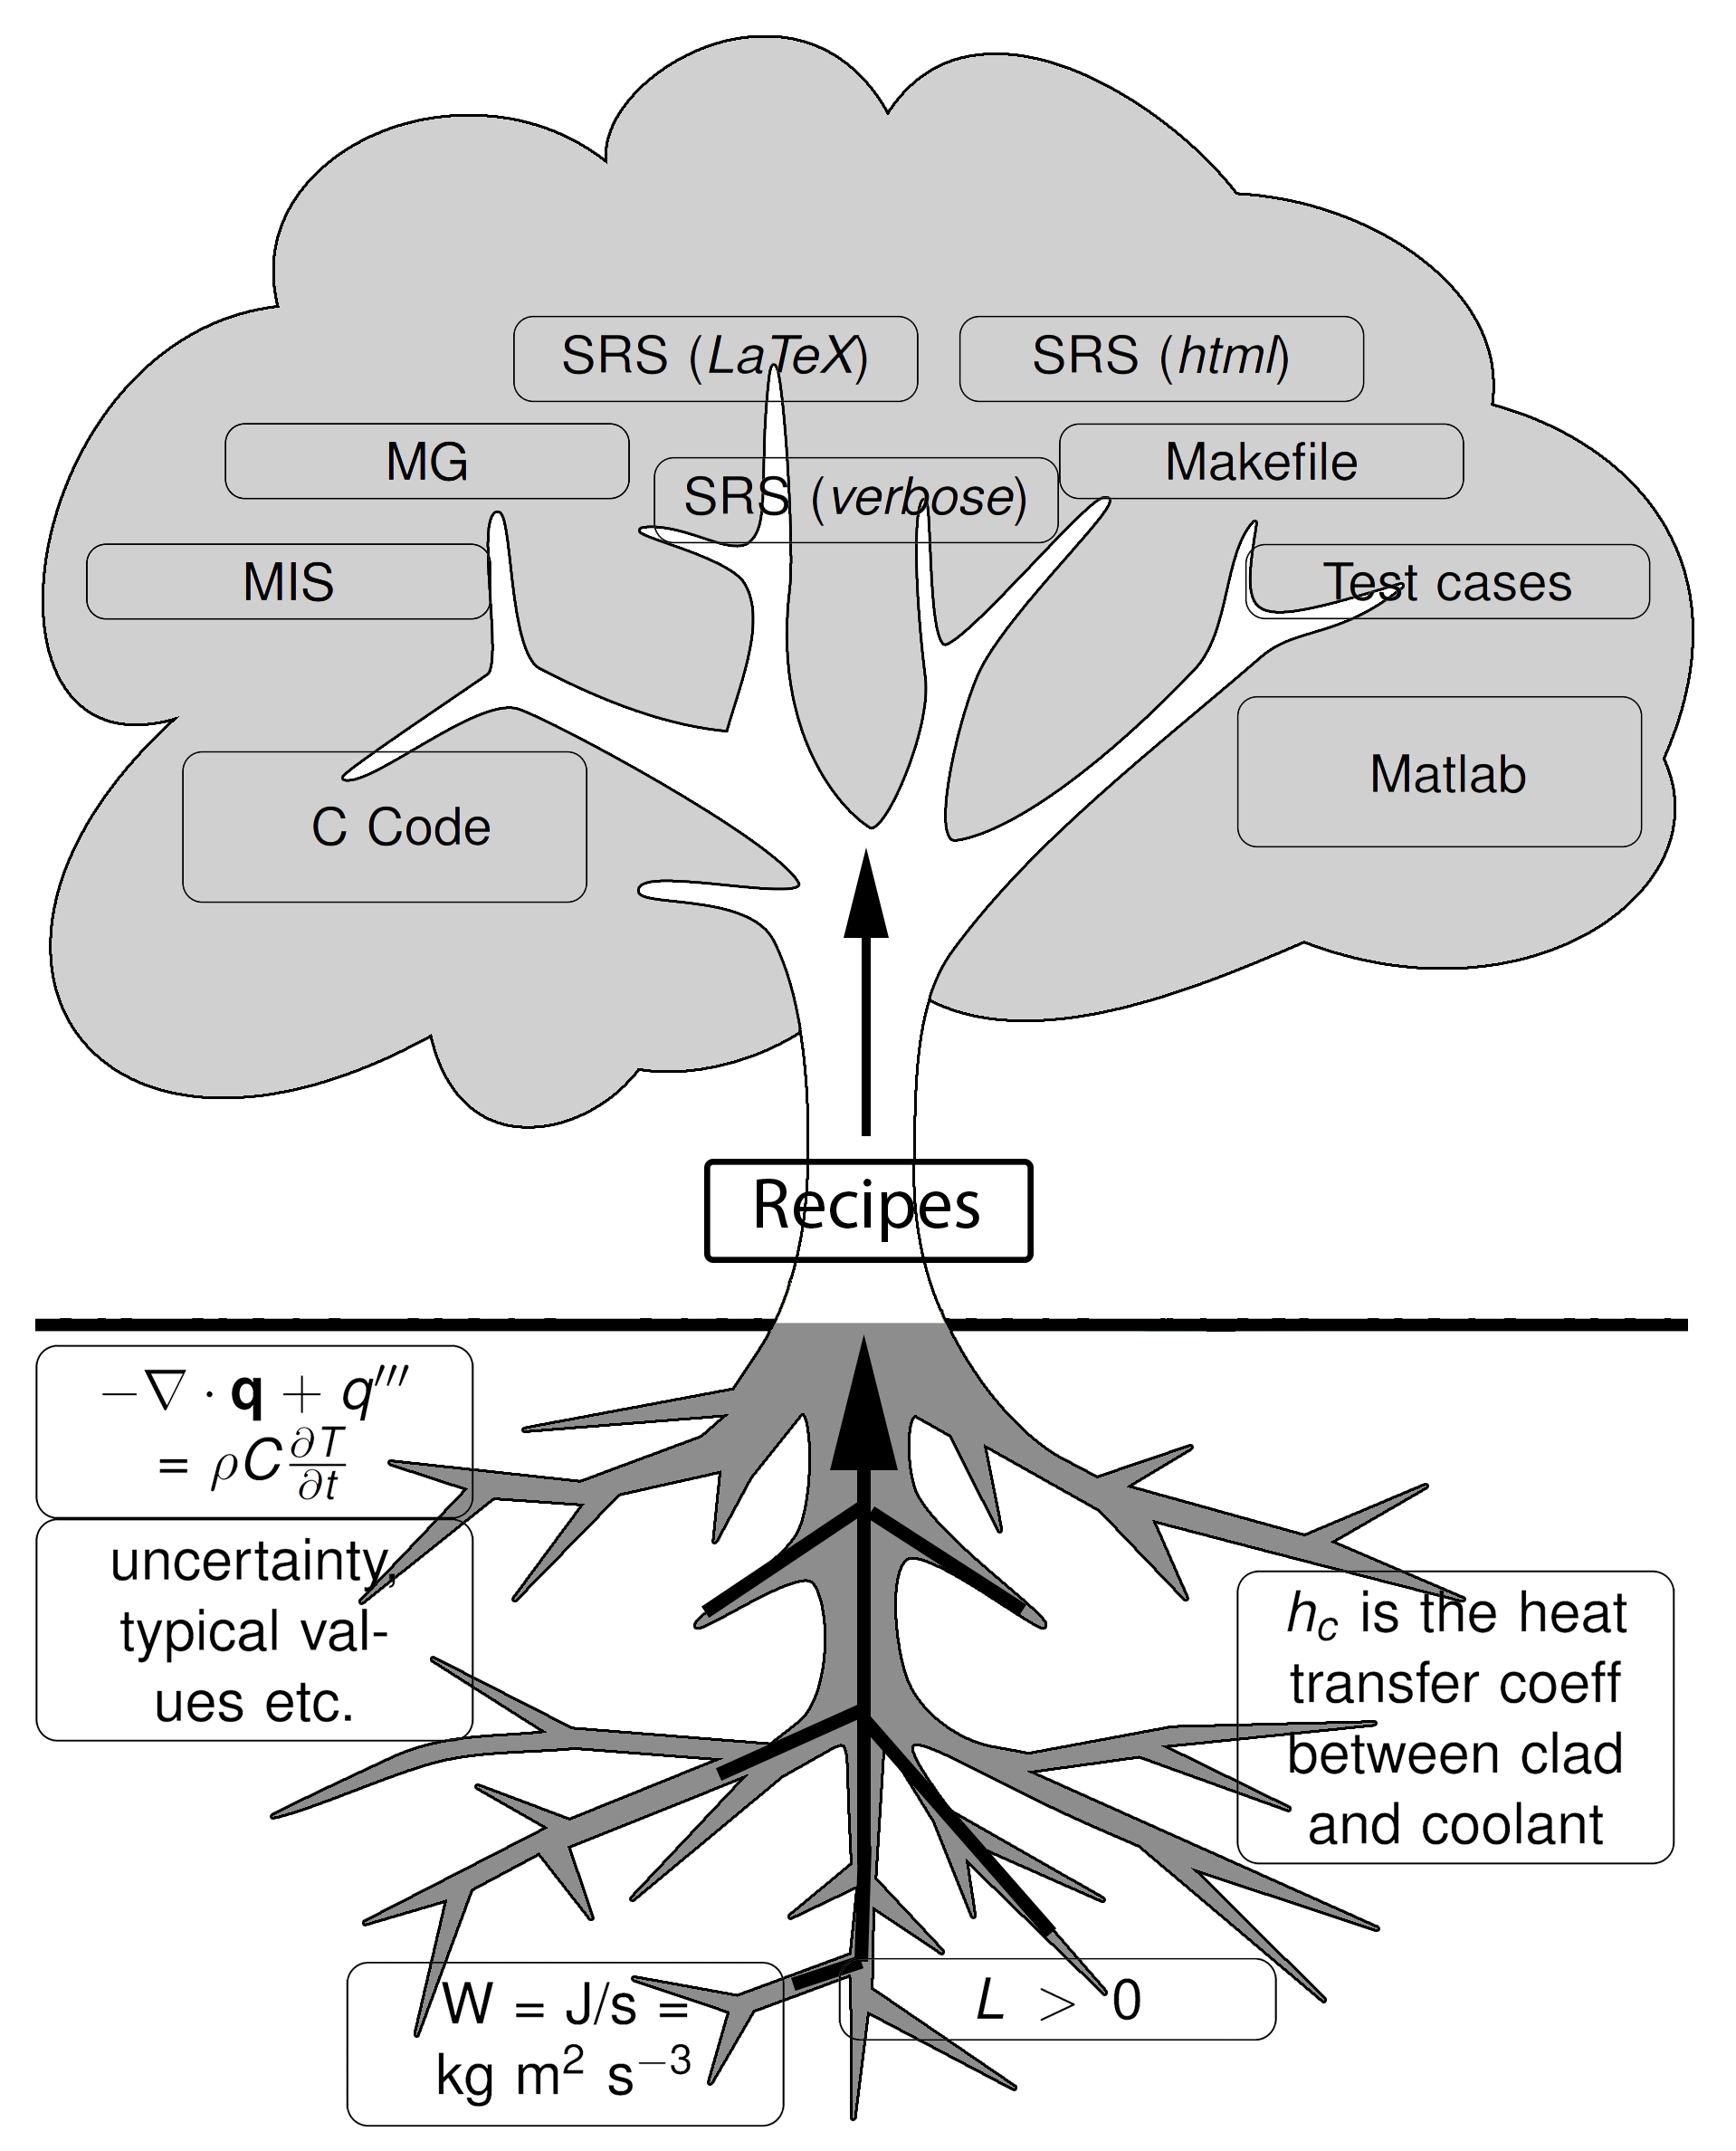
\includegraphics[height=20em]{tree.png}
\end{center}
}

\only<5>{
Drasil Framework
\begin{itemize}
\item Practical, example-driven approach %D Explain how this works!
\item Small case studies to start
\item Larger case studies in progress
\end{itemize}
}

\end{frame}

%%%%%%%%%%%%%%%%%%%%%%%%%%%%%%%%%%%%%

\subsection[Drasil]{The Drasil Framework}

%%%%%%%%%%%%%%%%%%%%%%%%%%%%%%%%%%%%%

\begin{frame}
\frametitle{Design}

Drasil is currently being implemented as a combination of six eDSLs:

\begin{itemize}
\item Expression
\item Expression Layout
\item Document Layout
\item C Representation
\item \LaTeX{} Representation
\item HTML Representation
\end{itemize}

\end{frame}

%%%%%%%%%%%%%%%%%%%%%%%%%%%%%%%%%%%%%

\begin{frame}
\frametitle{Chunks}

\begin{center}
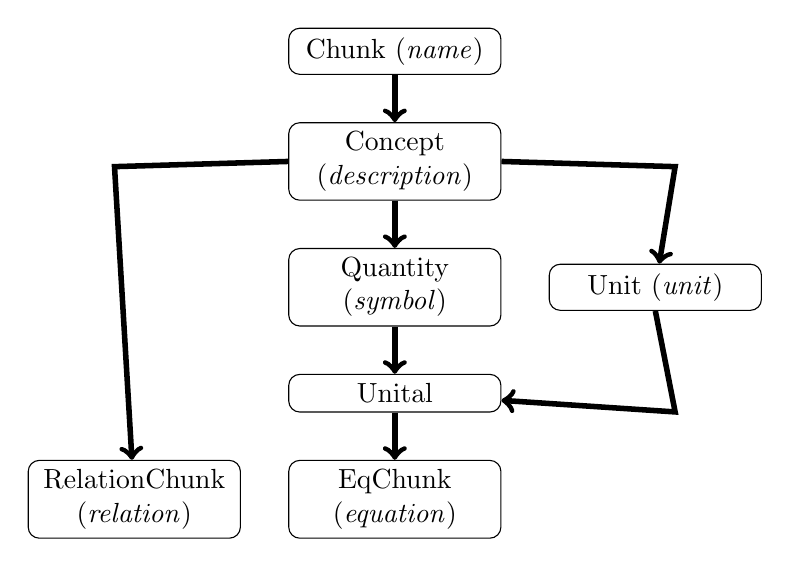
\begin{tikzpicture}[node distance=6mm]
  \tikzstyle{every node}=[draw,shape=rectangle, rounded corners,
    text width=7em, text centered];
  \node (ch)                     	{Chunk (\emph{name})};
  \node (co) [below = of ch]       {Concept (\emph{description})};
  \node (qu) [below = of co]  		{Quantity (\emph{symbol})};
  \node (u ) [right = of qu] 		{Unit (\emph{unit})};
  \node (uc) [below = of qu] 		{Unital};
  \node (eq) [below = of uc]	{EqChunk (\emph{equation})};
  \node (rc) [left = of eq]	{RelationChunk (\emph{relation})};

  \draw [->, line width=2pt] (ch) -- (co);
  \draw [->, line width=2pt] (co.west) -- (-3.56,-1.465) -- (rc); 
		%No idea how to do this
  \draw [->, line width=2pt] (co) -- (qu);
  \draw [->, line width=2pt] (co.east) -- (3.56,-1.465) -- (u );
  \draw [->, line width=2pt] (qu) -- (uc);
  \draw [->, line width=2pt] (u .south) -- (3.56,-4.58) -- (uc);
  \draw [->, line width=2pt] (uc) -- (eq);
\end{tikzpicture}
\end{center}

\end{frame}

%%%%%%%%%%%%%%%%%%%%%%%%%%%%%%%%%%%%%

\begin{frame}[fragile]
\frametitle{Example -- Fuel Pin SRS}

\href{run:SRS.pdf}{Original SRS from \LaTeX{}}

\href{run:gen_SRS.pdf}{SRS from Generated \LaTeX{}}

\href{run:gen_SRS.html}{Generated HTML SRS}

\end{frame}

%%%%%%%%%%%%%%%%%%%%%%%%%%%%%%%%%%%%%

\begin{frame}[fragile]
\frametitle{Example -- Recipes}

\only<1>{
\lstinputlisting[frame=single,firstline=13,basicstyle=\tiny]{HGHC.hs}
}

\only<2>{
\lstinputlisting[frame=single,basicstyle=\tiny]{Units.hs}
}

\end{frame}

\begin{frame}[fragile]
\frametitle{Example -- Chunks}

\lstinputlisting[frame=single,firstline=26,lastline=52,basicstyle=\tiny]{HeatTransfer.hs}

\end{frame}

%%%%%%%%%%%%%%%%%%%%%%%%%%%%%%%%%%%%%%%

\begin{frame}[fragile]
\frametitle{Example -- Common Knowledge}

\begin{lstlisting}[frame=single,showstringspaces=false, basicstyle=\tiny]
metre, second, kelvin, mole, kilogram, ampere, candela :: FundUnit
metre    = fund "Metre"    "length (metre)"               "m"
second   = fund "Second"   "time (second)"                "s"
kelvin   = fund "Kelvin"   "temperature (kelvin)"         "K"
mole     = fund "Mole"     "amount of substance (mole)"   "mol"
kilogram = fund "Kilogram" "mass (kilogram)"              "kg"
ampere   = fund "Ampere"   "electric current (ampere)"    "A"
candela  = fund "Candela"  "luminous intensity (candela)" "cd"
\end{lstlisting}

\end{frame}

%%%%%%%%%%%%%%%%%%%%%%%%%%%%%%%%%%%%%%%

\begin{frame}
\frametitle{Impressions}

\only<1>{
Advantages to a knowledge-based approach using Drasil:
\begin{enumerate}
\item No inconsistencies inter-/intra-artifact
\item Full traceability
\item Automatic update propagation
\item Reusable knowledge
\item Pervasive bugs
\end{enumerate}
}

\only<2>{
Disadvantages:
\begin{enumerate}
\item No local hacks
\item Creating common knowledge is difficult
\item Large short-term investment
\end{enumerate}
}
\end{frame}

%%%%%%%%%%%%%%%%%%%%%%%%%%%%%%%%%%%%%%%

\section[Next Steps]{Next Steps}

%%%%%%%%%%%%%%%%%%%%%%%%%%%%%%%%%%%%%%%

\begin{frame}

\frametitle{Next Steps}

Planned features:
\begin{itemize}
\item More types of information (i.e. physical constraints \& reasonable values)
\item Generate test cases from constraints
\item More output languages (MATLAB)
\item More artifact types
\item Different document views
\item External syntax
\end{itemize}

\end{frame}

%%%%%%%%%%%%%%%%%%%%%%%%%%%%%%%%%%%%%%%

\begin{frame}[allowframebreaks]

\frametitle{References}

\nocite{Roache1998, IonescuAndJansson2013, Kelly2007, CarverEtAl2007,
AckroydEtAl2008, EasterbrookAndJohns2009, Segal2005, Kelly2013, Kelly2015,
Owen1998, Merali2010, PatrickEtAl2015, Wilson2006, LoggEtAl2012,
KiselyovEtAl2004, Carette2006, PuschelEtAl2005, SmithAndKoothoor2016,
SmithEtAl2015-SS-TR, SmithEtAl2015SQJ, SmithEtAl2013, Knuth1984,
JohnsonAndJohnson1997, PieterseKourieAndBoake2004, ShumAndCook1993, Hyman1990,
Kotula2000, Thimbleby1986, Nedialkov2006, PharrAndHumphreys2004,
FritzsonGunnarssonAndJirstrand2002, Simonis2003, Ramsey1994, Leisch2002,
Mills1986, AlMatiiAndBoujarwah2002, Deck1996, SchulteEtAl2012,
GentlemanAndLang2012, LenthEtAl2007, Lenth2009, FlattEtAl2009}


\bibliography{drasil}

\end{frame}

\end{document}